\subsection{Дифференциал функции}

\begin{definition}
    Пусть $f: I \to \R$, $I$ -- промежуток, дифференцируема в точке $a$. Линейная функция $h \mapsto f'(a)h$, $h \in \R$, называется \textit{дифференциалом} функции $f$ в точке $a$ и обозначается $df_{a}$.
\end{definition}

Для функции $x \mapsto x$ функция $dx(h) = 1\cdot h$ в любой точке. Следовательно, $df_{a}(h) = f'(a)dx(h)$. Или в функцианальной записи: $df_{a}=f'(a)dx$.

\begin{note}
    Формулу из \hyperlink{th1}{Теоремы 1.1} можно переписать
    \[f(x) = f(a) + df_{a}(x-a)+o(x-a), x \to a\]
    \begin{center}
        \begin{tikzpicture}
            \draw[->] (-0.1,0) -- (3,0) node[below] {$x$};
            \draw[->] (0,0) -- (0,3) node[left] {$y$};
            \draw[very thick] (0,0) to [out=10, in=250] (2.5,2.3);
            \draw[very thick] (0.55,0) to [out=30, in=210] (3,1.7);
            \draw[very thick, dashed] (1.35,0) -- (1.35,0.5);
            \draw[very thick, dashed] (2,0) -- (2,1.32);
            \draw[very thick, dashed] (1.35,0.5) -- (2,0.5);
            \node at (3.5,1.8) {\color{red} $l_{\text{кас}}$};
            \node at (1.35,-0.2) {\color{red} $a$};
            \node at (2,-0.2) {\color{red} $x$};
            \node at (2.7,0.9) {\color{red} $df_{a}(h)$};
        \end{tikzpicture}
    \end{center}
\end{note}

\begin{corollary}
    В условиях \hyperlink{th2}{Теоремы 1.2}:
    \[d(\alpha f + \beta g)_{a} = \alpha d f_{a} + \beta d g_{a}\]
    \[d(f \cdot g)_{a} = g(a)df_{a} + f(a)dg_{a}\]
    \[d(\frac{f}{g})_{a} = \frac{g(a)df_{a}-f(a)dg_{a}}{g^{2}(a)}\]
\end{corollary}

\begin{corollary}
    В условиях \hyperlink{th3}{Теоремы 1.3}:
    \[d(g_{o}f)_{a} = (dg_{b})_{o}(df_{a})\]
\end{corollary}

\begin{proof}
    \[d(g_{o}f)_{a}(h) = g'(f(a))\cdot f'(a)dx(h)=g'(b)df_{a}(h) = dg_{b}(df_{a}(h)) \ \ \forall h \in \R\]
\end{proof}

\begin{note}{Инвариантность дифференциала.}\\
    Из доказательства следует, что формула
    \[df_{x} = f'(x)dx\]
    верна и в случае, когда $x$ -- независимая переменная, и в случае, когда $x = x(t)$.
\end{note}

\begin{corollary}
    В условиях \hyperlink{th4}{Теоремы 1.4} для обратной функции $f^{-1}$:
    \[d(f^{-1})_{b} = (df_{a})^{-1}\]
\end{corollary}

\begin{proof}
    $h \mapsto \frac{1}{f'(a)}h$ является обратной к функции $h \to f'(a)h$.
\end{proof}

\subsection{Теоремы о среднем.}

\begin{definition}
    Пусть $f$ определена на интервале, содержащем точку $a$.\\
    Точка $a$ называется \textit{точкой локального максимума (строгого)}, если 
    \[\exists \delta > 0 \ \ \forall x \in \mathring{B}_{\delta}(a) \ (f(x) \underset{(<)}{\leq} f(a))\]
    Аналогично определяются \textit{точки локального минимума (строгого)}.
\end{definition}

Точки локального максимума или минимума называются \textit{точками локального экстремума}.

\begin{example}

\end{example}
\begin{center}
    \begin{tikzpicture}
        \draw[->] (-3,0) -- (3,0) node[below] {$x$};
        \draw[->] (0,0) -- (0,3) node[left] {$y$};
        \draw[very thick] (0,0) to [out=10, in=250] (2,2);
        \draw[very thick] (-1,0.5) to [out=300, in=170] (0,0);
        \draw[very thick] (2,2) to [out=0, in=0] (2.5,2);
        \draw[very thick, dashed] (-1,0) -- (-1,0.48);
        \draw[very thick, dashed] (1,0) -- (1,0.48);
        \draw[very thick, dashed] (2,0) -- (2,2);
        \node at (-1,-0.2) {\color{red} $-1$};
        \node at (1,-0.2) {\color{red} $1$};
        \node at (2,-0.2) {\color{red} $2$};
    \end{tikzpicture}
\end{center}

Следующая теорема дает необходимое условие точки экстремума.

\begin{theorem}{Ферма}\\
    Пусть $f$ определена на интервале содержащем точку $a$.\\
    Если $a$ -- точка локального экстремума $f$ и $\exists f'(a)$, то $f'(a) = 0$.
\end{theorem}

\begin{proof}
    Пусть для определенности $a$ -- точка локального максимума. По определению:
    \[\exists \delta > 0 \ \ \forall x \in \mathring{B}_{\delta}(a) (f(x) \leq f(a)\]
    Тогда $\frac{f(x) - f(a)}{x - a} \leq 0$ на $(a, a + \delta) \Rightarrow f'(a) = f'_{+}(a) = \lim_{x \to a + 0}\frac{f(x) - f(a)}{x - a} \leq 0 \Rightarrow f'(a) \leq 0$.\\
    $\frac{f(x) - f(a)}{x - a} \geq 0$ на $(a - \delta, a) \Rightarrow f'(a) = f'_{-}(a) = \lim_{x \to a - 0}\frac{f(x) - f(a)}{x - a} \geq 0 \Rightarrow f'(a) \geq 0$.
    \\
    $\Rightarrow f'(a) = 0$
\end{proof}

\begin{note}{Геометрический смысл.}\\
    Если в точке экстремума существует касательная, то она горизонтальна.
\end{note}

\begin{theorem}{Ролль.}
    \begin{enumerate}
        \item $f$ -- непрерывна на $[a,b]$;
        \item $f$ -- дифференцируема на $(a,b)$;
        \item $f(a) = f(b)$;
    \end{enumerate}
    $\Rightarrow \exists c \in (a,b) \ (f'(c) = 0)$.
\end{theorem}

\begin{proof}
    По теореме Вейерштрасса $\exists x_{1}, x_{2} \in [a,b] \ (f(x_{1}) \leq f(x) \leq f(x_{2})) \ \ \forall x \in [a,b]$.
    Если $x_{1}, x_{2} \in \{a,b\}$ (концевые точки), то $f(x_{1})=f(x_{2}) \Rightarrow f$ постоянна на $[a,b]$. В качестве $c$ можно взять любую точку из $(a,b)$.
    \\
    Если $x_{1}, x_{2} \notin \{a,b\}$, то $\exists x_{i} \in (a,b)$. Тогда по теореме Ферма $f'(x_{i}) = 0$ и $c = x_{i}$.
\end{proof}

\begin{note}
    Геометрический смысл.
\end{note}

\begin{center}
    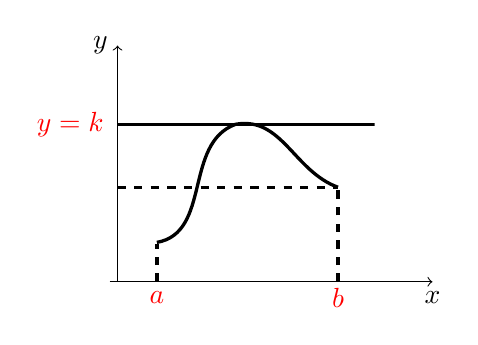
\begin{tikzpicture}
        \draw[->] (-0.1,0) -- (4,0) node[below] {$x$};
        \draw[->] (0,0) -- (0,3) node[left] {$y$};
        \draw[very thick] (0.5,0.5) to [out=10, in=200] (1.5,2) to [out=10, in=160] (2.8, 1.2);
        \draw[very thick] (0,2) to [out=0, in=0] (3,2);
        \draw[very thick, dashed] (0.5,0) -- (0.5,0.48);
        \draw[very thick, dashed] (2.8,0) -- (2.8,1.18);
        \draw[very thick, dashed] (0,1.2) -- (2.8,1.2);
        \node at (0.5,-0.2) {\color{red} $a$};
        \node at (2.8,-0.2) {\color{red} $b$};
        \node at (-0.6,2) {\color{red} $y = k$};
    \end{tikzpicture}
\end{center}

\begin{corollary}
    Если $f$ дифференцируема на промежутке $I$, то между любыми двумя нулями $f$ существует хотя бы один нуль производной.
\end{corollary}

\begin{theorem}\hypertarget{lagrange}{Лагранж.}
    \begin{enumerate}
        \item $f$ -- непрерывна на $[a,b]$;
        \item $f$ -- дифференцируема на $(a,b)$;
    \end{enumerate}
    $\Rightarrow \exists c \in (a,b) \ (f(b) - f(a) = f'(c)(b-a))$
\end{theorem}

\begin{proof}
    Рассмотрим $h(x) = f(x) - \frac{f(b) - f(a)}{b - a}(x - a) - f(a)$. Тогда $h$ -- непрерывна на $[a,b]$, $h$ -- дифференцируема на $(a,b)$ и $h(a) = 0 = h(b)$.\\
    Следовательно, по теореме Ролля, $\exists c \in (a,b) \ h'(c) = 0 \lra f'(c) - \frac{f(b) - f(a)}{b - a} = 0$.
\end{proof}

\begin{note}{Геометрический смысл.}\\
    $f'(c) = \frac{f(b) - f(a)}{b - a}$.
    \begin{center}
        \begin{tikzpicture}
            \draw[->] (-0.1,0) -- (3,0) node[below] {$x$};
            \draw[->] (0,0) -- (0,3) node[left] {$y$};
            \draw[very thick] (0.5,0.5) to [out=80, in=190] (2.5,2.5);
            \draw[very thick, ->] (0.5,0.5) to [out=45, in=225] (2.5,2.5);
            \draw[very thick] (0.5,1.2) to [out=45, in=225] (2.5,3.2);
            \draw[very thick, dashed] (0.5,0) -- (0.5,0.5);
            \draw[very thick, dashed] (2.5,0) -- (2.5, 2.5);
            \draw[very thick, dashed] (1.18,0) -- (1.2,1.9);
            \node at (3,3.2) {\color{red} $l_{\text{кас}}$};
            \node at (0.5,-0.2) {\color{red} $a$};
            \node at (2.5,-0.2) {\color{red} $b$};
            \node at (1.18,-0.2) {\color{red} $c$};
        \end{tikzpicture}
    \end{center}
    Найдется точка $c$ в которой касательная параллельна хорде.
\end{note}

\begin{problem}\hypertarget{task1} \ \\
    Пусть \begin{enumerate}
        \item $f$ - непрерывна на $[a, b)$
        \item $f$ - дифференцируема на $(a, b)$
        \item $\exists \ f'(a+0)$
    \end{enumerate}
    Тогда $f_+'(a) = f'(a+0)$.
\end{problem}

\begin{corollary}{Оценка приращения функции.}\\
    Пусть $f$ -- непрерывна на промежутке $I$ и дифференцируема на $int(I)$.\\
    Если $f'(x)$ ограничена на $int(I)$, т.е. $\exists c > 0 \ \forall x \in int(I) \ (|f'(x)| < c)$, то 
    \[\forall x,y \in I \ (|f(y) - f(x)| \leq c|y-x|)\]
    (т.е. $f$ -- липшицева). В частности, $f$ раномерно непрерывна на $I$.
\end{corollary}

\begin{proof}
    Пусть $x, y \in I \ (x \neq y)$. Тогда по теореме Лагранжа $f(y) - f(x) = f'(c)(y - x)$ для некоторой $c \in (x, y)$. Так как $c \in int(I)$, то $|f'(c)| \leq C$ и, значит, $|f(y) - f(x)| \leq c|y - x|$.
\end{proof}

\begin{theorem}\hypertarget{koshi_o_srednem}{Коши.}
    \begin{enumerate}
        \item $f, g$ -- непрерывны на $[a,b]$;
        \item $f, g$ -- дифференцируемы на $(a,b)$;
        \item $g \neq 0$ на $(a,b)$;
    \end{enumerate}
    $\Rightarrow \exists c \in (a,b) \ (\frac{f(b) - f(a)}{g(b) - g(a)} = \frac{f'(c)}{g'(c)})$.
\end{theorem}

\begin{proof}
    Отметим, что $g(b) \neq g(a)$, иначе, по теореме Ролля, $\exists \psi \in (a,b) \ (g(\psi) = 0)$. Рассмотрим $h(x)=f(x) - \frac{f(b) - f(a)}{g(b) - g(a)}(g(x) - g(a)$. Тогда $h$ -- непрерывна на $[a,b]$ и дифференцируема на $(a,b)$ и $h(a) = h(b) = f(a)$. По теореме Ролля:
    \[\exists c \in (a,b) \ h'(c) = 0 \ \lra \ f'(c) = \frac{f(b) - f(a)}{g(b) - g(a)}g'(c) = 0.\]
    Так как $g'(c) \neq 0$, то $\frac{f(b) - f(a)}{g(b) - g(a)} = \frac{f'(c)}{g'(c)}$.
\end{proof}

\begin{note}{Геометрический смысл.}\\
    Геометрический смысл теоремы Коши такой же, как и для теоремы Лагранжа, применённой к параметрически заданной функции:
    $\begin{cases}
        x = f(t),\\
        y = g(t),
    \end{cases}$
    $t \in [a,b]$.
    Поскольку в теореме Ферма предполагается лишь существование производной, то Т6, Т7, Т8 остаются справедливы при замене дифференцируемости функций на существование производных в $\overline{\R}$.
\end{note}